% Options for packages loaded elsewhere
\PassOptionsToPackage{unicode}{hyperref}
\PassOptionsToPackage{hyphens}{url}
\PassOptionsToPackage{dvipsnames,svgnames,x11names}{xcolor}
%
\documentclass[
  10pt,
  ignorenonframetext,
]{beamer}
\usepackage{pgfpages}
\setbeamertemplate{caption}[numbered]
\setbeamertemplate{caption label separator}{: }
\setbeamercolor{caption name}{fg=normal text.fg}
\beamertemplatenavigationsymbolsempty
% Prevent slide breaks in the middle of a paragraph
\widowpenalties 1 10000
\raggedbottom
\setbeamertemplate{part page}{
  \centering
  \begin{beamercolorbox}[sep=16pt,center]{part title}
    \usebeamerfont{part title}\insertpart\par
  \end{beamercolorbox}
}
\setbeamertemplate{section page}{
  \centering
  \begin{beamercolorbox}[sep=12pt,center]{part title}
    \usebeamerfont{section title}\insertsection\par
  \end{beamercolorbox}
}
\setbeamertemplate{subsection page}{
  \centering
  \begin{beamercolorbox}[sep=8pt,center]{part title}
    \usebeamerfont{subsection title}\insertsubsection\par
  \end{beamercolorbox}
}
\AtBeginPart{
  \frame{\partpage}
}
\AtBeginSection{
  \ifbibliography
  \else
    \frame{\sectionpage}
  \fi
}
\AtBeginSubsection{
  \frame{\subsectionpage}
}
\usepackage{amsmath,amssymb}
\usepackage{lmodern}
\usepackage{iftex}
\ifPDFTeX
  \usepackage[T1]{fontenc}
  \usepackage[utf8]{inputenc}
  \usepackage{textcomp} % provide euro and other symbols
\else % if luatex or xetex
  \usepackage{unicode-math}
  \defaultfontfeatures{Scale=MatchLowercase}
  \defaultfontfeatures[\rmfamily]{Ligatures=TeX,Scale=1}
\fi
\usetheme[]{Singapore}
\usefonttheme{serif}
% Use upquote if available, for straight quotes in verbatim environments
\IfFileExists{upquote.sty}{\usepackage{upquote}}{}
\IfFileExists{microtype.sty}{% use microtype if available
  \usepackage[]{microtype}
  \UseMicrotypeSet[protrusion]{basicmath} % disable protrusion for tt fonts
}{}
\makeatletter
\@ifundefined{KOMAClassName}{% if non-KOMA class
  \IfFileExists{parskip.sty}{%
    \usepackage{parskip}
  }{% else
    \setlength{\parindent}{0pt}
    \setlength{\parskip}{6pt plus 2pt minus 1pt}}
}{% if KOMA class
  \KOMAoptions{parskip=half}}
\makeatother
\usepackage{xcolor}
\newif\ifbibliography
\usepackage{graphicx}
\makeatletter
\def\maxwidth{\ifdim\Gin@nat@width>\linewidth\linewidth\else\Gin@nat@width\fi}
\def\maxheight{\ifdim\Gin@nat@height>\textheight\textheight\else\Gin@nat@height\fi}
\makeatother
% Scale images if necessary, so that they will not overflow the page
% margins by default, and it is still possible to overwrite the defaults
% using explicit options in \includegraphics[width, height, ...]{}
\setkeys{Gin}{width=\maxwidth,height=\maxheight,keepaspectratio}
% Set default figure placement to htbp
\makeatletter
\def\fps@figure{htbp}
\makeatother
\setlength{\emergencystretch}{3em} % prevent overfull lines
\providecommand{\tightlist}{%
  \setlength{\itemsep}{0pt}\setlength{\parskip}{0pt}}
\setcounter{secnumdepth}{-\maxdimen} % remove section numbering
\newlength{\cslhangindent}
\setlength{\cslhangindent}{1.5em}
\newlength{\csllabelwidth}
\setlength{\csllabelwidth}{3em}
\newlength{\cslentryspacingunit} % times entry-spacing
\setlength{\cslentryspacingunit}{\parskip}
\newenvironment{CSLReferences}[2] % #1 hanging-ident, #2 entry spacing
 {% don't indent paragraphs
  \setlength{\parindent}{0pt}
  % turn on hanging indent if param 1 is 1
  \ifodd #1
  \let\oldpar\par
  \def\par{\hangindent=\cslhangindent\oldpar}
  \fi
  % set entry spacing
  \setlength{\parskip}{#2\cslentryspacingunit}
 }%
 {}
\usepackage{calc}
\newcommand{\CSLBlock}[1]{#1\hfill\break}
\newcommand{\CSLLeftMargin}[1]{\parbox[t]{\csllabelwidth}{#1}}
\newcommand{\CSLRightInline}[1]{\parbox[t]{\linewidth - \csllabelwidth}{#1}\break}
\newcommand{\CSLIndent}[1]{\hspace{\cslhangindent}#1}
\setbeamertemplate{navigation symbols}{}
\setbeamertemplate{footline}[page number]
\usepackage{tcolorbox}
\ifLuaTeX
  \usepackage{selnolig}  % disable illegal ligatures
\fi
\IfFileExists{bookmark.sty}{\usepackage{bookmark}}{\usepackage{hyperref}}
\IfFileExists{xurl.sty}{\usepackage{xurl}}{} % add URL line breaks if available
\urlstyle{same} % disable monospaced font for URLs
\hypersetup{
  pdftitle={Best practices in data analysis},
  pdfauthor={Stefanie Muff},
  colorlinks=true,
  linkcolor={Maroon},
  filecolor={Maroon},
  citecolor={Blue},
  urlcolor={blue},
  pdfcreator={LaTeX via pandoc}}

\title{Best practices in data analysis}
\subtitle{Selecting a model}
\author{Stefanie Muff}
\date{Open Science course, Finse, November 2022}

\begin{document}
\frame{\titlepage}

\begin{frame}
\begin{block}{Introduction and overview}
\protect\hypertarget{introduction-and-overview}{}
\(~\)

\begin{itemize}
\tightlist
\item
  ``Best practices in data analysis'' is a huge field.
\end{itemize}

\(~\)

\begin{itemize}
\tightlist
\item
  Today: some words on model selection.
\end{itemize}
\end{block}
\end{frame}

\begin{frame}
\begin{block}{Developing a model}
\protect\hypertarget{developing-a-model}{}
\(~\)

In statistics courses, the correct models often ``fall from heaven'':
The model family and the terms in the model were almost always given.

\(~\)

However, it is often not immediately obvious which terms are relevant to
include in a model.

\(~\)

Importantly, the approach to find a model \textbf{heavily depends on the
aim} for which the model is built.\\
\(~\)

The following distinction is important:

\begin{itemize}
\tightlist
\item
  The aim is to \alert{predict} future values of \(y\) from known
  regressors.
\item
  The aim is to \alert{explain} \(y\) using known regressors.
  Ultimately, the aim is to \emph{find causal relationships}.
\end{itemize}
\end{block}
\end{frame}

\begin{frame}
\(\rightarrow\) Even among statisticians there is no real consensus
about how, if, or when to select a model:


\includegraphics{graphics/brewer_title.jpg}
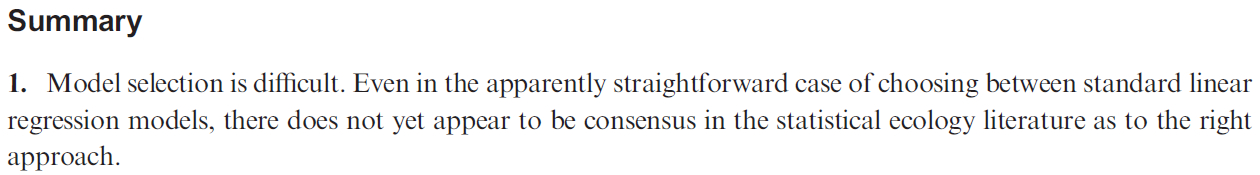
\includegraphics{graphics/brewer.jpg}

Note: The first sentence of a paper in \emph{Methods in Ecology and
Evolution} from 2016 is: ``Model selection is difficult.'\,'
\end{frame}

\begin{frame}
Why is finding a model so hard?

\(~\)

Note that a model is only an \emph{approximation} to reality. The aim of
a data analysis is to understand something about the real world thanks
to \emph{simplifications}.

\(~\)

Box (1979): \textbf{``All models are wrong, but some are useful.'\,'}

\(~\)

\(\rightarrow\) There is often not a ``right'' or a ``wrong'' model --
but there are more and less useful ones.

\(\rightarrow\) Finding a model with good properties is sometimes an
art\ldots{}
\end{frame}

\begin{frame}
\begin{block}{Two examples}
\protect\hypertarget{two-examples}{}
\(~\)

\begin{enumerate}
\tightlist
\item
  \textbf{Understanding the effect of mercury (Hg) in the soil}
  \emph{Research question:} Is the Hg level in the environment (soil) of
  people's homes associated to the Hg levels in their bodies (urin,
  hair)?\\
  \emph{Method:} Measurements of Hg concentrations on people's
  properties, as well as measurements and survey of children and their
  mothers living on these properties.
\end{enumerate}

\(~\)

\begin{enumerate}
\setcounter{enumi}{1}
\tightlist
\item
  \textbf{Prognostic factors for body fat}\\
  \emph{Research question:} Which factors allow for precise estimation
  (prediction) of body fat?\\
  \emph{Method:} Study with 241 male participants. Measured variable
  were, among others, body fat (\%), age, weight, body size, BMI, neck
  thickness and abdominal girth.
\end{enumerate}
\end{block}
\end{frame}

\begin{frame}
\begin{block}{Predictive and explanatory models}
\protect\hypertarget{predictive-and-explanatory-models}{}
\(~\)

Before we continue to discuss model/variable selection, we need to be
clear about the scope of the model:

\(~\)

\begin{itemize}
\tightlist
\item
  \textcolor{red}{Predictive models}: These are models that aim to
  predict the outcome of future subjects.\\
  \textbf{Example:} In the bodyfat example the aim is to predict
  people's bodyfat from factors that are easy to measure (age, BMI,
  weight,..).
\end{itemize}

\(~\)

\begin{itemize}
\tightlist
\item
  \textcolor{red}{Explanatory models}: These are models that aim at
  understanding the (causal) relationship between covariates and the
  response.\\
  \textbf{Example}: The mercury study aims to understand if
  Hg-concentrations in the soil (covariable) influence the
  Hg-concentrations in humans (response).
\end{itemize}

\(~\)

\(\rightarrow\) The model selection strategy depends on this
distinction.
\end{block}
\end{frame}

\begin{frame}
\begin{block}{Prediction vs explanation}
\protect\hypertarget{prediction-vs-explanation}{}
\(~\)

\begin{quote}
When the aim is \textcolor{red}{prediction}, the best model is the one
that best predicts the fate of a future subject. This is a well defined
task and ``objective'' variable selection strategies to find the model
which is best in this sense are potentially useful.
\end{quote}

\(~\)

\begin{quote}
However, when used for \textcolor{red}{explanation} the best model will
depend on the scientific question being asked, and \textbf{automatic
variable selection strategies have no place}.
\end{quote}

\(~\)

\scriptsize (Clayton and Hills 1993)
\end{block}
\end{frame}

\begin{frame}
\begin{block}{Model selection for predictive models}
\protect\hypertarget{model-selection-for-predictive-models}{}
\(~\)

\begin{itemize}
\tightlist
\item
  Cross-validation (CV)
\end{itemize}

\(~\)

\begin{itemize}
\tightlist
\item
  AIC, BIC, DIC, \ldots{}
\end{itemize}

\(~\)

\begin{itemize}
\tightlist
\item
  If you want, even forward and backward selection is ok.
\end{itemize}

\(~\)

\begin{itemize}
\tightlist
\item
  Any (other) optimization procedure of some ``cost function''.
\end{itemize}
\end{block}
\end{frame}

\begin{frame}
\begin{block}{Model selection for explanatory models?}
\protect\hypertarget{model-selection-for-explanatory-models}{}
\(~\)

\begin{tcolorbox}
Model selection may lead to biased parameter estimates, thus do not draw (biological, medical,..) conclusions from models that were optimized for prediction, for example by AIC/AICc/BIC minimization!
\end{tcolorbox}

\(~\) \scriptsize See, e.g., (Freedman 1983) and (Copas 1983).
\end{block}
\end{frame}

\begin{frame}
\(~\)

``Explanation'' means that you will want to interpret the regression
coefficients, 95\% CIs and \(p\)-values. It is then often assumed that
some sort of causality (\(x\rightarrow y\)) exists.

\(~\)

In such a situation, you should formulate a
\textcolor{red}{confirmatory model}:

\(~\)

\begin{tcolorbox}
\begin{itemize}
\item Start with a {\bf clear hypothesis.}

\vspace{2mm}

\item Select your covariates according to {\bf a priori knowledge.}

\vspace{2mm}

\item Ideally, formulate {\bf only one} or a few model(s) {\bf before you start analysing your data}.
\end{itemize}

\end{tcolorbox}

\vspace{8mm}

You might consider \emph{pre-registration}.
\end{frame}

\begin{frame}
Confirmatory models have a long tradition medicine. In fact, the main
conclusions in a study are only allowed to be drawn from the main model
(which needs to be specified even before data are collected):

\vspace{2mm}

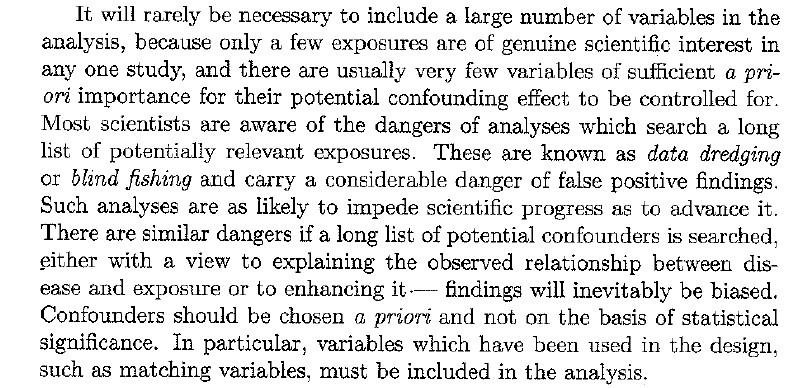
\includegraphics[width=0.9\textwidth,height=\textheight]{graphics/claytonHills.jpg}
\(~\)

\scriptsize (Clayton and Hills 1993)
\end{frame}

\begin{frame}
\begin{block}{Model selection bias -- coded example}
\protect\hypertarget{model-selection-bias-coded-example}{}
\(~\)

\url{https://github.com/stefaniemuff/statlearning/tree/master/OpenScience/bestPracticeAnalysis/Rcode_exercise}

\(~\)

\begin{tcolorbox}
{\bf Aim of the example:} \\
To illustrate how model selection purely based on AIC can lead to biased parameters and overestimated effects.

\end{tcolorbox}
\end{block}
\end{frame}

\begin{frame}
\begin{block}{Confirmatory vs.~exploratory}
\protect\hypertarget{confirmatory-vs.-exploratory}{}
\(~\)

Any \emph{additional analyses} that you potentially do with your data
have the character of \emph{exploratory models}.

\vspace{2mm}

\(\rightarrow\) Two sorts of explanatory models/analyses:

\vspace{2mm}

\textcolor{red}{Confirmatory}:

\begin{tcolorbox}

\begin{itemize}
\item Clear hypothesis and a priori  selection of regressors for the response. 
\item No variable selection! 
\item Allowed to interpret the results and draw quantitative conclusions.  
\end{itemize}

\end{tcolorbox}

\pause

\textcolor{red}{Exploratory}:

\begin{tcolorbox}
\begin{itemize}
\item Build whatever model you want, but the results should only be used to generate new hypotheses, a.k.a. ``speculations''.
 \item Clearly label the results as ``exploratory''.
\end{itemize}
    
\end{tcolorbox}
\end{block}
\end{frame}

\begin{frame}
\begin{block}{Summary}
\protect\hypertarget{summary}{}
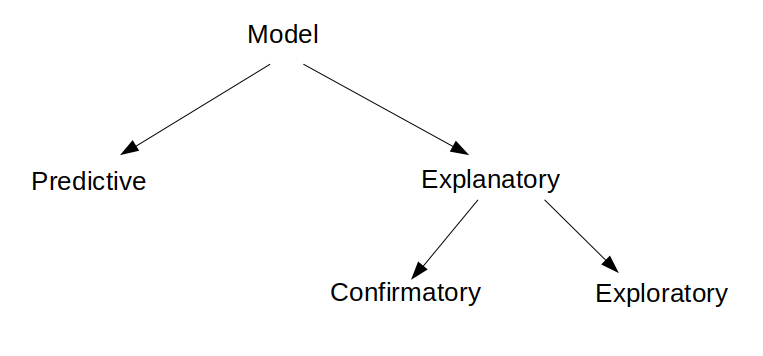
\includegraphics{graphics/models.png}
\end{block}
\end{frame}

\begin{frame}{References}
\protect\hypertarget{references}{}
\scriptsize

\hypertarget{refs}{}
\begin{CSLReferences}{1}{0}
\leavevmode\vadjust pre{\hypertarget{ref-clayton.hills1993}{}}%
Clayton, D., and M. Hills. 1993. \emph{Statistical Models in
Epidemiology}. Oxford: Oxford University Press.

\leavevmode\vadjust pre{\hypertarget{ref-copas1983}{}}%
Copas, J. B. 1983. {``Regression, Prediction and Shrinkage.''}
\emph{Journal of the Royal Statistical Society. Series B (Statistical
Methodology)} 45: 311--54.

\leavevmode\vadjust pre{\hypertarget{ref-freedman1983}{}}%
Freedman, D. A. 1983. {``A Note on Screening Regression Equations.''}
\emph{The American Statistician} 37: 152--55.

\end{CSLReferences}
\end{frame}

\end{document}
